\documentclass[twocolumn]{article}
\usepackage{url}
\usepackage{titling}
\usepackage{graphicx}
\usepackage{hyperref}
\usepackage[utf8]{inputenc}
\usepackage{array,etoolbox}
\usepackage[none]{hyphenat}
\usepackage[justification=centering]{caption}
\usepackage[acronym,nomain,nonumberlist,nogroupskip,nopostdot]{glossaries}

% loads the list of abbreviations
\makeglossaries
\loadglsentries{acronym}

% centers the title page
\renewcommand\maketitlehookd{\vfill\null}
\renewcommand\maketitlehooka{\null\mbox{}\vfill}

% keywords command
\providecommand{\keywords}[1]
{
	\small
	\noindent \textbf{\textit{Keywords ---}} #1
}

% counter for table
\preto\tabular{\setcounter{magicrownumbers}{0}}
\newcounter{magicrownumbers}
\newcommand\rownumber{\stepcounter{magicrownumbers}\arabic{magicrownumbers}}

% use an alias for the model names
\newcommand{\mobilenet}{MobileNetV2}
\newcommand{\xception}{Xception}
\newcommand{\inception}{InceptionV3}
\newcommand{\resnet}{InceptionResNetV2}


\begin{document}


\setlength{\droptitle}{-5cm}
\title{\textbf{\gls{asl}\\
	Fingerspelling Detection}}
\author{Shoaib Mohammed}
\date{01 July 2021}
\maketitle


\begin{abstract}
Approximately 70 million people around the world are deaf-mute. While 
translation services have become easily accessible for about 100 
languages, sign language is still an area that has not been explored. 
Our goal is to detect \& translate the letters of \gls{asl} in real-time.
\end{abstract}

\keywords{\gls{asl}, fingerspelling, \gls{cnn}, transfer learning, 
computer vision}


\section{Introduction}

\subsection{Background}
According to the \gls{csd} \cite{csd}, there are 360 million deaf people 
worldwide. Another report by the \gls{who} \cite{who} bumps up the number to 
466 million people or over 6\% of the world's population suffering from 
disabling hearing loss. But even in this age of technology and communication, 
we are yet to see a universal translation system that helps bridge the gap 
between people that can and cannot speak. \gls{asl} is a natural language 
meaning it was not created and was spread by the people who employ the signs 
by the movement of hands, facial expressions, and body posture. The goal of 
this project is to detect and accurately translate the letters in \gls{asl}.

% (TODO: cite image to the website https://qualityansweringservice.com/american-sign-language-guide/)
\begin{figure}[h]
\centering
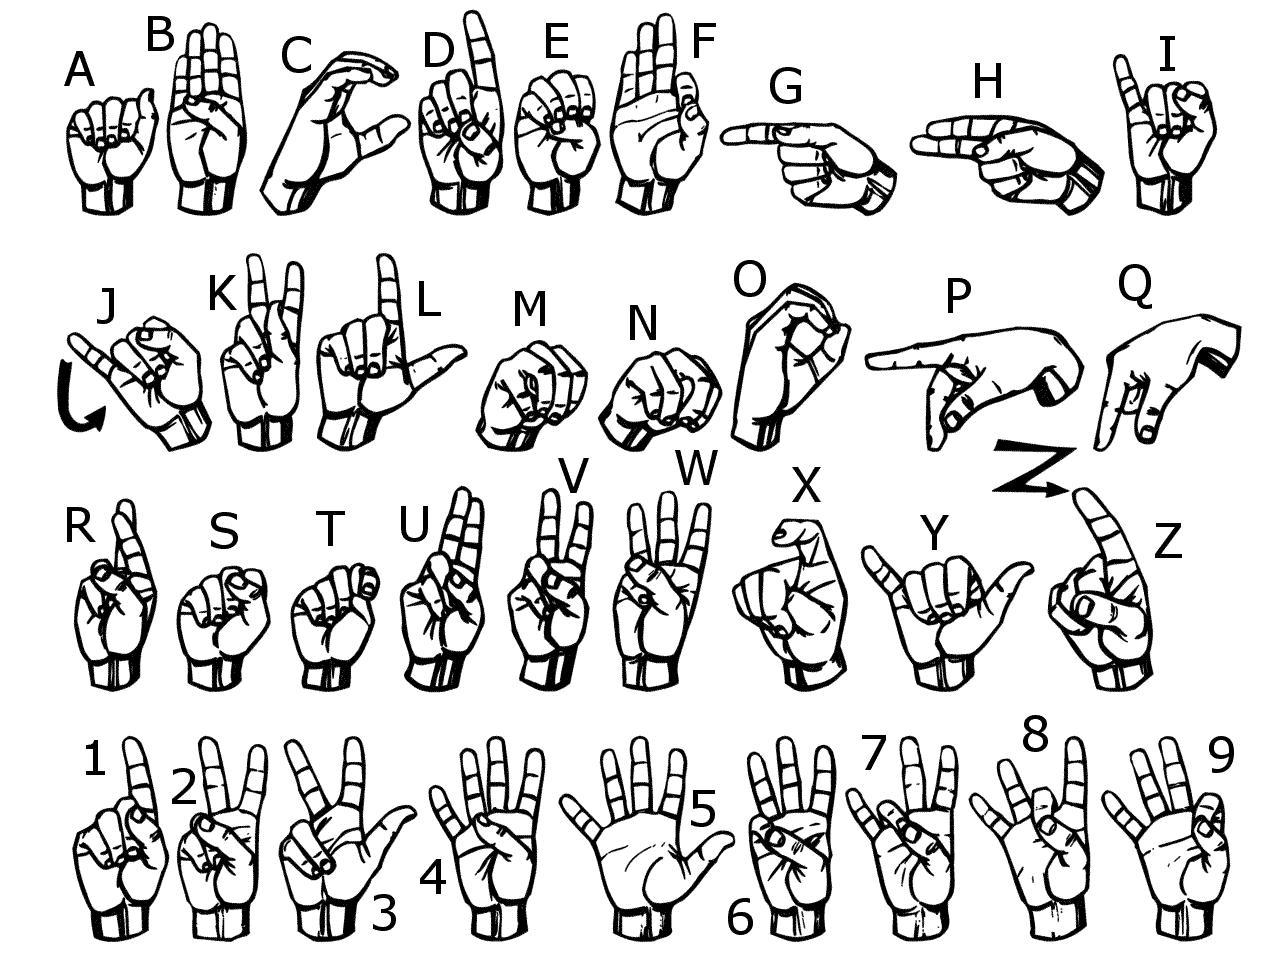
\includegraphics[width=8cm]{./figures/asl alphabets}
\caption{Alphabets in \gls{asl}}
\label{asl alphabets}
\end{figure}

\subsection{Geographical Distribution}

The true count for the number of sign languages is still unknown given the 
vast majority, however, \textit{Ethnologue} \cite{ethnologue} lists this 
number to be \textit{137} \cite{fenlon2015sign}. Given the vast majority, 
\gls{asl} is still the most popular sign language and is being widely used 
around the globe. In addition to being the primary source of communication for 
a sign language in the United States, \gls{asl} is being used throughout most 
of the provinces in Canada \cite{al2010sign}.

\begin{figure}[h]
\centering
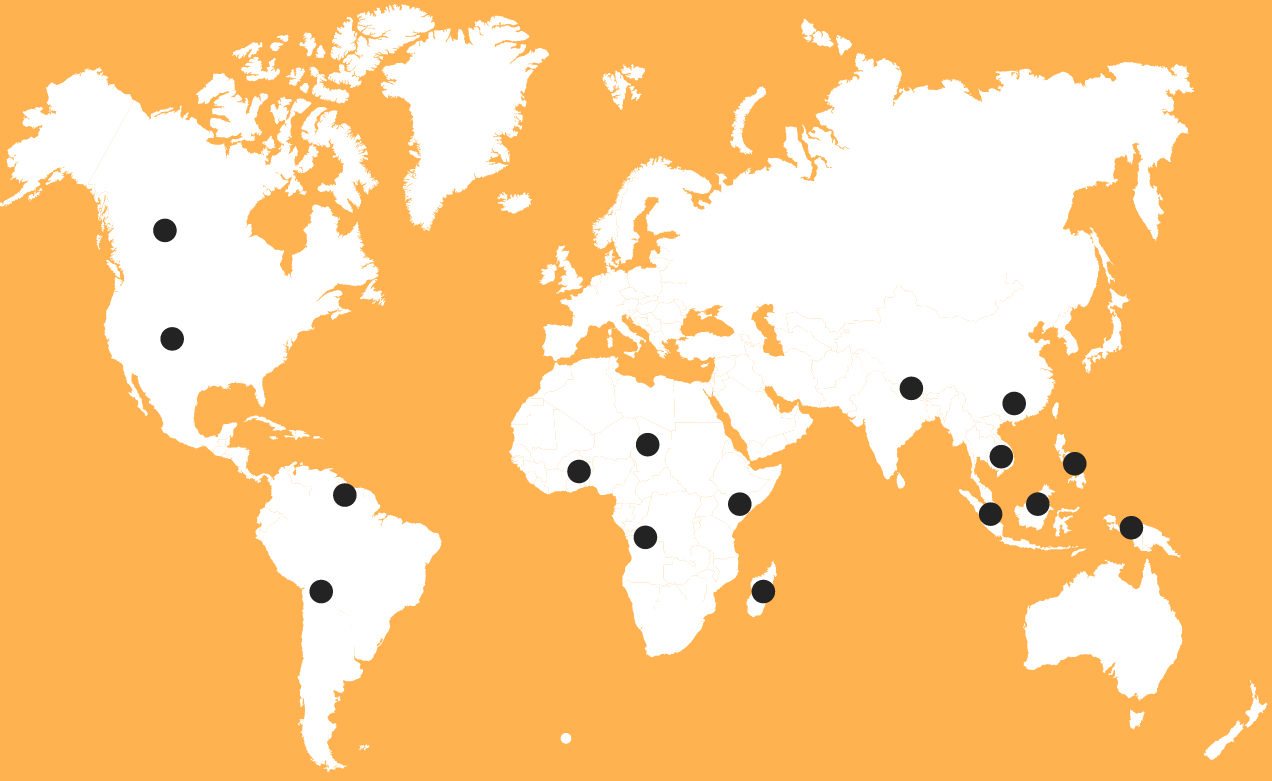
\includegraphics[width=8cm]{./figures/asl being used around the world}
\caption{ASL being used around the world}
\end{figure}

Variations of \gls{asl} are also being used worldwide. Sign language 
similar to \gls{asl} is being used throughout Africa in places such as 
Nigeria, Ghana, Guyana, Central African Republic, Jamaica, Zimbabwe, and 
Kenya \cite{nyst2010sign}.

\subsection{Scope \& Limitations}

% (TODO: do we want to add acronyms for US & UK?)
The bottom line is that there is no universal sign language. For instance, the 
\gls{bsl} differs by a great margin from \gls{asl}, this is clear when 
comparing \autoref{asl alphabets} with \autoref{bsl alphabets}. Generally 
speaking, a person in the US can understand spoken English in the UK but this 
is not the case with sign language. Even though there is a multitude of sign 
languages being used across the world, if an accurate model was developed to 
recognize a sign language, in our case, \gls{asl}, the same methodology could 
be applied to recognize other sign languages.

% (TODO: cite image to the website https://universeofmemory.com/british-sign-language-resources/)
\begin{figure}[h]
\centering
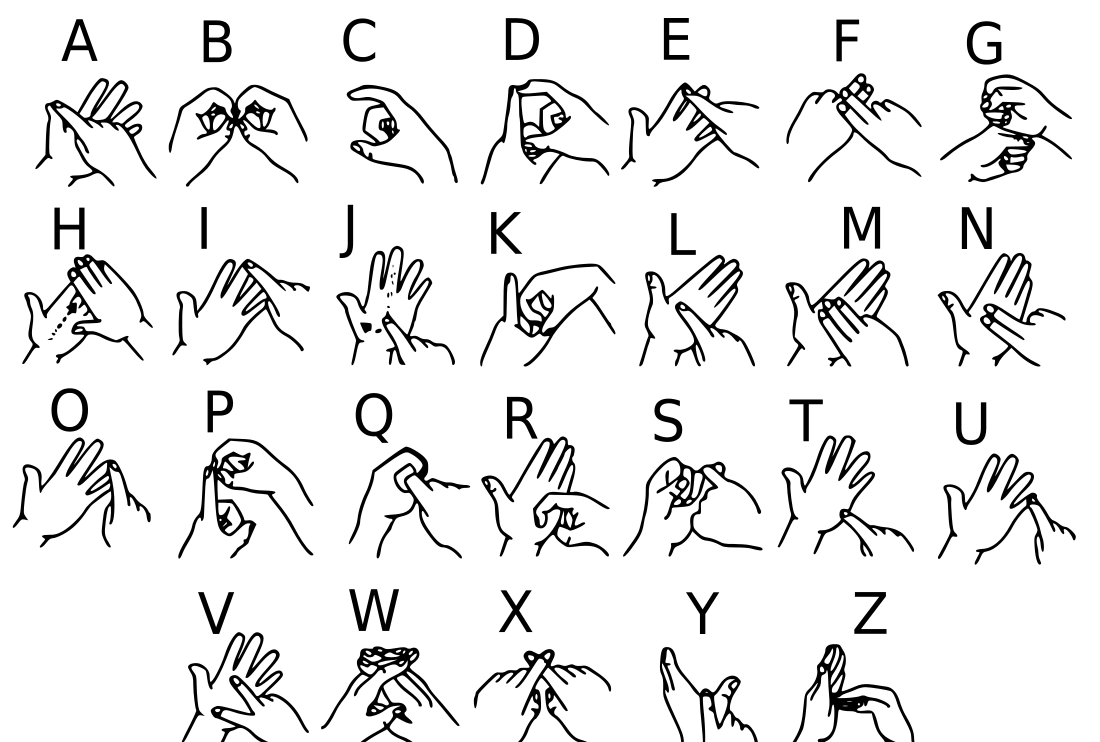
\includegraphics[width=8cm]{./figures/bsl alphabets}
\caption{Alphabets in \gls{bsl}}
\label{bsl alphabets}
\end{figure}

One big limitation for classification is that most signs require motion and 
are not static. Even more so as there are signs which are formed by the same 
motion but the repetition or the number of times a motion is repeated differs. 
Things get even more challenging as facial expressions are important in sign 
languages which is akin to the vocal tone of a person's voice when speaking. 
Two signs may be exactly the same visually but the face gesture of the signer 
makes them different.

Perhaps the major limitation is classifying each sign from the sheer corpus of 
signs in \gls{asl}. A dictionary on \gls{asl} contains illustrations for more 
than \textit{1,600} signs \cite{tennant1998american}. However, our focus is 
classifying the alphabets alone which limits our range to \textbf{24} 
alphabets since we exclude the alphabets J \& Z because these require motion.

\section{Literature Survey}

\subsection{Population Statistics}
A combined study in \cite{mitchell2006many} estimates there were more than 
250,000 deaf people and as many as 500,000 people who used \gls{asl} in 1972. 
Over the years, this number has been on the rise. Based on their research for 
in year 2006, fewer than 1 in 20 Americans or 10,000,000 people suffered from 
\textit{hard of hearing} and close to 1,000,000 were classified as 
\textit{functionally deaf}.

\begin{figure}[h]
\centering
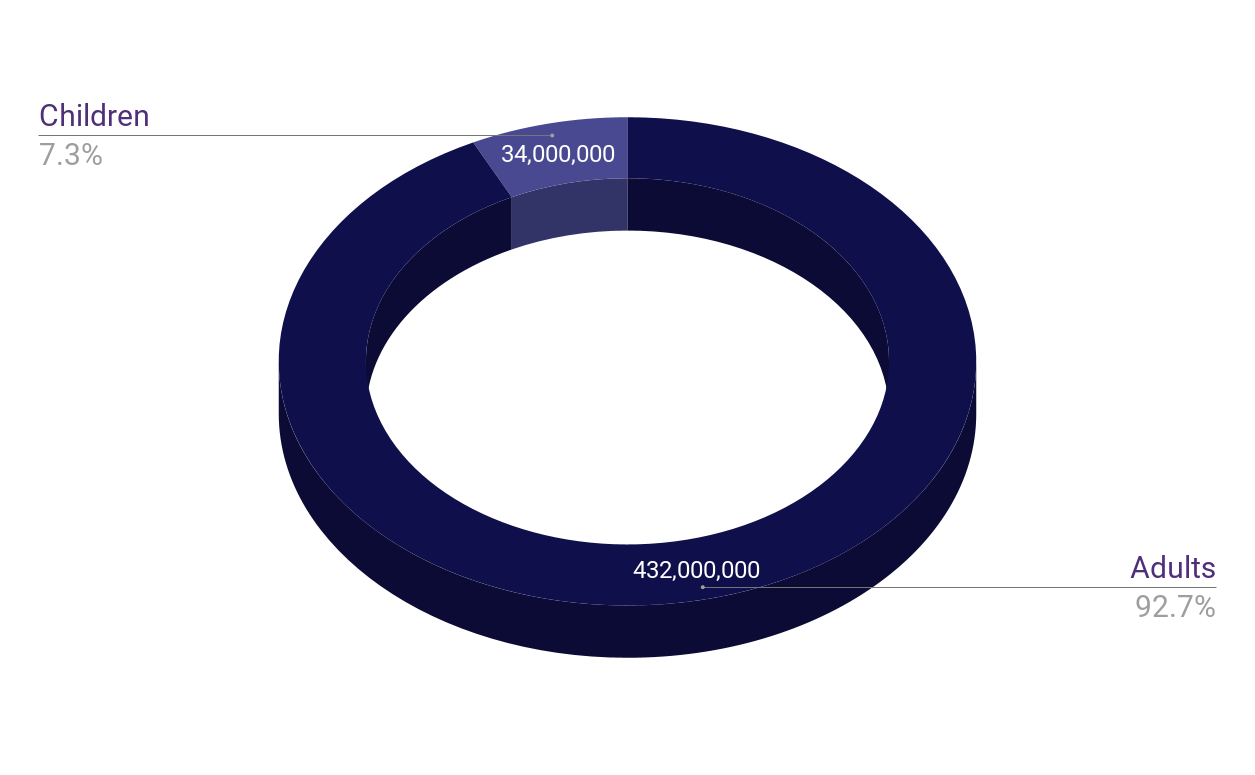
\includegraphics[width=8cm]{./figures/distribution of the population}
\caption{Distribution of the population}
\end{figure}

In 2016, the \gls{nidcd} \cite{nidcd} released statistics about hearing loss 
in the United States. About 2 to 3 out of every 1,000 children have hearing 
loss. Approximately 15\% of adults (37.5 million) aged 18 and over report 
trouble hearing and 18\% of adults aged 20-69 have speech-frequency hearing 
loss in both ears. Furthermore, about 2\% of adults aged 45-54, 8.5\% of 
adults aged 55-64, 25\% of adults aged 65-74, and 5\% of adults aged 75 and 
older have disabling hearing loss.

In terms of the distribution of people suffering from hearing loss \cite{who}, 
432 million people are adults and 34 million are children. Future projections 
estimate 630 million people by 2030 and over 900 million people by 2050.

\subsection{Existing Models}

There has been ongoing research in this area with the growth in machine 
learning and datasets being made available publicly. Many of the models use 
Kinect to recognize the hand gestures and map them to \gls{asl}.

Earlier versions of work used a sensory glove. In 2005, Cemil and Ming 
\cite{oz2005recognition} worked on recognizing the alphabets in \gls{asl} by 
using a sensory Cyberglove and a motion tracker to extract the gestures. By 
processing the data of the fingers on the strain gauges, the trajectory, and 
orientation from the motion tracker through an \gls{ann}, high accuracy 
results were achieved. Building upon this in 2011, Cemil and Ming 
\cite{oz2011american} used feature extraction with noise reduction and were 
able to classify 50 ASL words. A similar approach was used in 2014 
\cite{patil2014american} where the output of the sensor glove gets sent to a 
microcontroller through an \gls{adc}. The glove uses flex sensors which 
capture the bending of each finger. The predicted letter gets displayed on an 
LCD. Although this worked well, it is impractical in real-life. The whole 
system requires several high components to be connected each time someone 
needs to sign a letter.

% (TODO: cite image to the website http://www.cyberglovesystems.com/)
\begin{figure}[h]
\centering
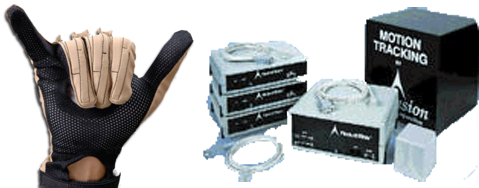
\includegraphics[width=8cm]{./figures/cyberglove and flock of birds}
\caption{Cyberglove and Flock of Birds by Ascension}
\end{figure}

Due to the sophisticated components required by using sensor gloves, there's 
been lots of research on translating ASL by using depth cameras. In 2015, we 
had a major breakthrough successfully translating the 24 static \gls{asl} 
alphabet signs using a Microsoft Kinect \cite{dong2015american}. A latex 
color glove allowed for easier hand segmentation and localizing the joint 
positions. The prediction was done through a \gls{rf} classifier on the depth 
data. The Kinect has also been used in conjunction with hidden Markov 
models \cite{lang2012sign} for recognition. Even with good results, the Kinect 
is not something people just carry around. Furthermore, depth cameras are also 
known to perform badly under poor lighting conditions.

% (TODO: cite image to the reference \cite{dong2015american}
% paper https://openaccess.thecvf.com/content_cvpr_workshops_2015/W15/papers/Dong_American_Sign_Language_2015_CVPR_paper.pdf)
\begin{figure}[h]
\centering
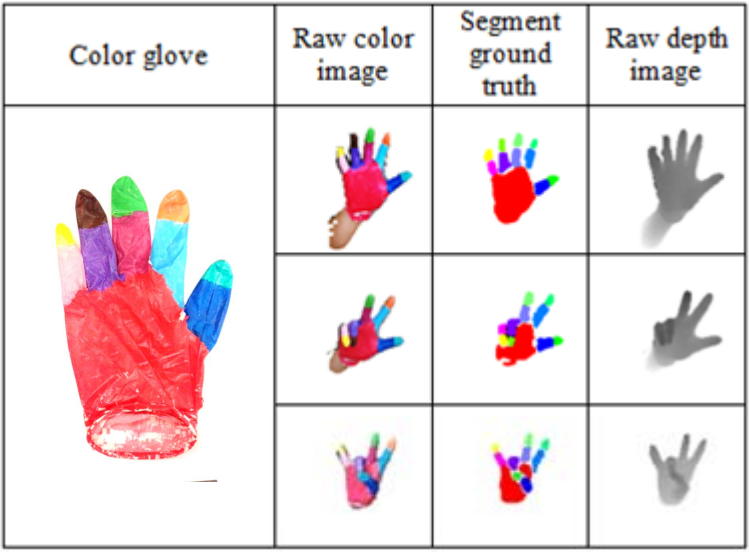
\includegraphics[width=8cm]{./figures/color glove}
\caption{A color glove allowed easier hand segmentation}
\end{figure}

In 2015, a hand gesture recognition model was developed using depth and 
intensity channels with 3D \gls{cnn} \cite{molchanov2015hand}. A similar 
methodology was used to recognize sign language by extracting spatio-temporal 
features \cite{huang2015sign}. To improve the performance, multi-channels of 
video streams including color, depth, and body joint information are used as 
input to the 3D \gls{cnn}. In 2017, a features extractor with deep behavior 
was used to deal with the Arabic Sign Language \cite{elbadawy2017arabic}. By 
combining the features extractor with a 3D \gls{cnn}, the recognition system 
was fed with data from depth maps and could recognize 25 gestures.

% (TODO: cite image to the reference paper "Explaining hyperspectral imaging based plant disease identification: 3D CNN and saliency maps"
% paper https://www.researchgate.net/publication/324744613_Explaining_hyperspectral_imaging_based_plant_disease_identification_3D_CNN_and_saliency_maps)
\begin{figure}[h]
\centering
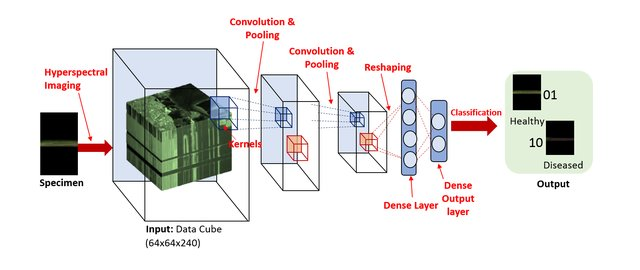
\includegraphics[width=8cm]{./figures/3d cnn}
\caption{3D Convolutional Neural Network}
\end{figure}

In 2018 a different solution was proposed, SignFi \cite{ma2018signfi} which 
uses Wi-Fi to recognize sign language. SignFi can recognize 276 gestures 
involving the head, arm, hand, and finger gestures with high accuracy. SignFi 
works based on \gls{csi} which describes how a signal propagates from the 
transmitter to the receiver at a certain carrier frequency. SignFi uses Wi-Fi 
packets as input and a 9-layer \gls{cnn} as the classification algorithm.

Realizing the challenges faced by the above mentioned methods, our goal is to 
create a machine learning model with transfer learning to classify the 
alphabets of \gls{asl} in real-time. By using \textit{four} transfer learning 
models, namely, \mobilenet \cite{sandler2018mobilenetv2}, 
\xception \cite{chollet2017xception}, \inception \cite{szegedy2016rethinking}, 
and \resnet \cite{szegedy2017inception}, we achieve a high accuracy.

\section{Problem Description}

\subsection{Data Gathering}

Looking for available datasets, the \textit{\gls{asl} Finger Spelling Dataset} 
\cite{pugeault2011spelling} is perhaps the most popular one. There were others 
too, but they did pose a few problems. There were many outliers present in the 
dataset including the faces of the subjects. This causes difficulties while 
training the model since our focus is the hand. The other datasets which focus 
on the hand contain less outliers but do not contain a lot of variation 
causing the model to overfit. Hence, we decided to create our own dataset 
fixing the aforementioned problems by focusing on the hand and adding 
variation by using more subjects in different locations.

% (TODO: cite image to the reference \cite{pugeault2011spelling}
% paper https://openaccess.thecvf.com/content_cvpr_workshops_2015/W15/papers/Dong_American_Sign_Language_2015_CVPR_paper.pdf)
\begin{figure}[h]
\centering
\includegraphics[width=8cm]{./figures/outliers in asl}
\caption{Outliers present in \gls{asl} Fingerspelling dataset \cite{pugeault2011spelling}}
\end{figure}

Using \texttt{python}, a helper script was created to generate data to train 
the model and has the following features:
\begin{itemize}
	\item Subjects: 5 different people with varying skin colors and features
	\item Shape: [250×250×3] having reasonable parameters for the input image
	\item Variability: taken with both good \& bad lighting
	\item Size: 4,000 images for each alphabet for a total 96,000 images
\end{itemize}

\begin{figure}[h]
\centering
\includegraphics[width=8cm]{./figures/asl fingerspelling}
\caption{ASL alphabets from our dataset}
\end{figure}

% (TODO: do we need this section?)
\subsection{Dependencies}

% (TODO: add the actual version numbers)
We have used the following dependencies:
\begin{itemize}
	\item \href{https://www.python.org/downloads/}{Python 3}
	\item \href{https://www.scipy.org/install.html}{Numpy}
	\item \href{https://keras.io/#installation}{Keras}
	\item \href{https://github.com/Kaggle/kaggle-api}{Kaggle API}
	\item \href{https://www.tensorflow.org/install}{TensorFlow}
\end{itemize}

All the codebase is written in the \texttt{python} programming language due to 
its wide support for machine learning algorithms with many different packages.

\subsection{Data Preparation}

% (TODO: this is a bit irrelevant and can be removed)
The first step is to define the labels which in our case is a set of
categorical labels. A helper script was created to accomplish just this task 
alone, given a string representing a set of labels it creates a 
\texttt{mapping.json} file with each label representing a numeric value. Due 
to the amount of data being processed for the model, it takes time to load and 
pre-process all of it. We can speed things up by using a common technique 
called \textit{serialization}. Serialization is the process of converting an 
object into a stream of bytes and saving that in the binary format in memory. 
When required, we can load this stream of bytes back as our object, this 
process is called \textit{deserialization}. Serialization allows us to have 
faster training as preprocessing the dataset on each run can take time. In 
\texttt{python}, serialization is commonly referred to as \textit{pickling}.

% (TODO: cite image to the website https://www.javatpoint.com/serialization-in-java)
\begin{figure}[h]
\centering
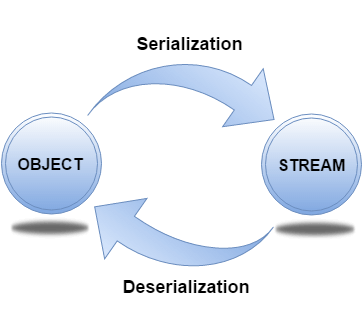
\includegraphics[width=8cm]{./figures/serialization and deserialization}
\caption{Process of serialization \& deserialization}
\end{figure}

The preprocessing phase consists of 3 parts:
\begin{enumerate}
	\item Load the data – We load the \texttt{xs} which is a list of images each 
	representing the pixel values in RGB format and the \texttt{ys} which is a 
	list of labels each representing the alphabet. We can load the images using 
	OpenCV which is a popular computer vision library.
	\item Preprocess the data – The input image size may not match the size 
	required as input for the model. We resize all the images to the shape 
	\texttt{[SHAPE × SHAPE × CHANNELS]} where the constants are collected from a 
	configuration file, it is also a good idea to one-hot encode the labels. 
	Lastly, it is recommended to shuffle the data since in the case of the data 
	being organized together, it may hinder the learning process of the model 
	during training.
	\item Split the data – We need to divide the data into train and test sets. 
	There is a common split called the \textit{80/20 split} which is derived 
	from the Pareto principle. This means 80\% of the data or 76,800 images are 
	used for the training set and the rest 20\% of the data or 19,200 images are 
	used for the testing set.
\end{enumerate}

\subsection{Configuration}

There are certain parameters that can be tweaked by the user to fit to his needs:
\begin{itemize}
	\item Epochs: number of passes through the training set, \textit{default = 64}.
	\item Shape: the shape of the square image, \textit{default = 250}.
	\item Channels: number of color channels, \textit{default = 3}.
	\item Batch Size: number of training samples used in one iteration, \textit{default = 128}.
\end{itemize}

\subsection{Transfer Learning}

We have used transfer learning to get a foundation for the model 
configuration. Transfer learning makes use of knowledge gained while solving 
one problem and applying it to a different but related problem. It is a 
popular approach in deep learning as it provides a strong foundation and a 
starting point given the vast amount of time and resources required to solve 
the related problem from scratch. In our case, we will use transfer learning 
models that have been trained to recognize patterns in images. As we are 
focusing on fingerspelling \gls{asl}, we do not require motion (since we 
exclude \textit{J \& Z} making it a related problem of finding patterns.

% (TODO: cite image to the website https://medium.datadriveninvestor.com/introducing-transfer-learning-as-your-next-engine-to-drive-future-innovations-5e81a15bb567)
\begin{figure}[h]
\centering
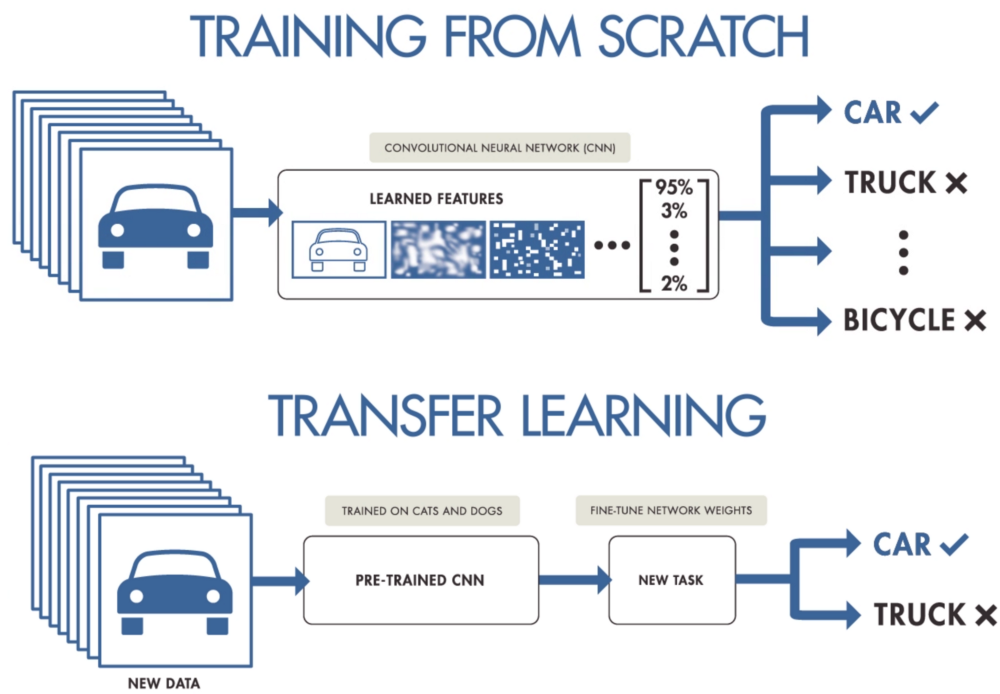
\includegraphics[width=8cm]{./figures/training from scratch vs. transfer learning}
\caption{Training from scratch vs. transfer learning}
\end{figure}

The \texttt{python} framework \texttt{keras} has many available models to 
choose, we have made available the following:
\begin{itemize}
	\item \mobilenet: lightweight and fast model that runs on a smartphone
	\cite{sandler2018mobilenetv2}
	\item \xception: deep \gls{cnn} with depth-wise separable convolutions
	\cite{chollet2017xception}
	\item \inception: refined from GoogLeNet with batch normalization and 
	factorization \cite{szegedy2016rethinking}
	\item \resnet: variation of \inception by adding residual connections and a 
	simplified architecture \cite{szegedy2017inception}
\end{itemize}

These were chosen carefully due to their ability to perform well on images and 
computer vision related tasks.

% (TODO: cite image to the website https://medium.com/@lorenzofamiglini/transfer-learning-with-deep-learning-machine-learning-techniques-b4052befe7e2)
\begin{figure}[h]
\centering
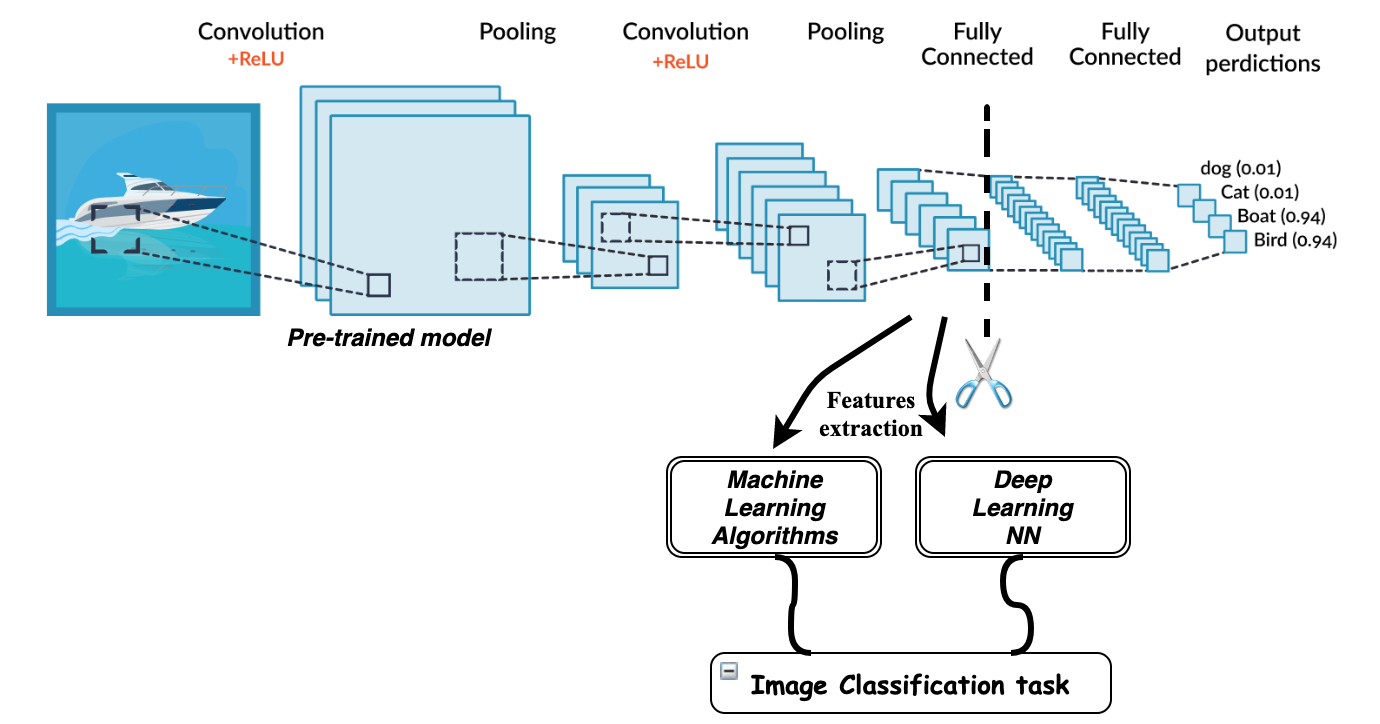
\includegraphics[width=8cm]{./figures/transfer learning process}
\caption{Transfer learning process}
\end{figure}

We pass the image as input to our transfer learning which is well-trained to 
figure out \textit{patterns}. The last layer in each transfer learning model 
is used to get the model’s prediction of the category/label. We will be using 
the 2\textsuperscript{nd} last layer which contains the activations of the 
transfer learning model.

Getting the activations of the transfer learning model takes time, hence, we 
store the model's activations on the entire dataset by using the technique of 
serialization as mentioned previously. These can be huge and consume memory, 
if space is an issue, then it’s better to compromise with longer training 
times.

\subsection{Model Architecture}

% (TODO: this can be removed as its relevant)
Keras allows two ways to create models:
\begin{itemize}
	\item \textit{Sequential}: allows to create a layer-by-layer model where the 
	inputs flow straight down to the output.
	\item \textit{Functional}: connect a given layer to any other layer 
	resulting in complex networks thus providing flexibility.
\end{itemize}

We use the \texttt{Sequential} model since we do not need to manually define 
and connect each layer of our model.

% (TODO: I don't think we should be explaining concepts in a research paper)
Next, we need to define our layers. Each layer in our network tries to build 
onto the work extracted from the previous layer. Layers extract useful 
information from the data fed into them. The goal is to have meaningful 
representations for our problem. Take a problem of recognizing parts of a 
human face from a selfie. The first layer may extract the person from the 
background. The second layer may extract parts of the human body from the 
person such as the arms, legs, face and so on. The third layer may extract 
parts of the face itself like the eyes, nose, mouth, hair and ears. The fourth 
layer may extract more in-depth features such as the wrinkles, dark circles, 
dimples and more. The activation function is used to decide which features are 
relevant. Essentially, by deciding if a neuron fires (activates) or not, we 
evaluate the importance of a feature in affecting the overall output.

Working on large images can be a problem. For example, take a high-resolution 
color image of width \texttt{1080 px} and height \texttt{720 px}. Since a 
color image contains 3 channels (RGB), the total number of parameters is 
\texttt{1080×720×3=2,332,800} parameters just for the input image alone! As we 
keep adding more layers, the number of parameters goes on increasing. It is 
recommended not to exceed 10 million parameters for the entire model as this 
can have computation issues as well as other known issues like over-fitting.

% (TODO: cite image to the website https://www.quora.com/What-is-the-benefit-of-using-average-pooling-rather-than-max-pooling)
\begin{figure}[h]
\centering
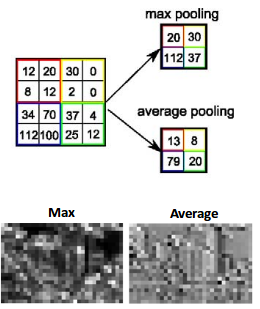
\includegraphics[width=8cm]{./figures/max pooling vs. average pooling}
\caption{Max pooling vs. Average pooling}
\end{figure}

A resolve to decrease the number of parameters is a technique called pooling. 
Pooling layers allow us to downsample our feature map by summarizing the 
features. For image data, max pooling tends to work better because there could 
be some extreme and important features (like edges) which get smoothened out 
in average pooling. These two common pooling methods are described below: 
\begin{itemize}
	\item Average Pooling: replaces each patch by its average value.
	\item Max Pooling: replaces each patch by its max value.
\end{itemize}

Before passing the output to the final layer which is a fully-connected layer, 
it is a good idea to flatten this output. The flatten layer unrolls the input 
to a single long one-dimensional array. Most of the work has been done at this 
point by all the previous layers in our model allowing us to figure out the 
patterns that are present. The work left now is to figure out the label, in 
our case, the \gls{asl} alphabet. We use fully-connected layers to help link 
the processed features together and predict the label.

% (TODO: cite image to the website https://medium.com/analytics-vidhya/understanding-a-single-neurons-role-in-neural-network-77bb3251e9db)
\begin{figure}[h]
\centering
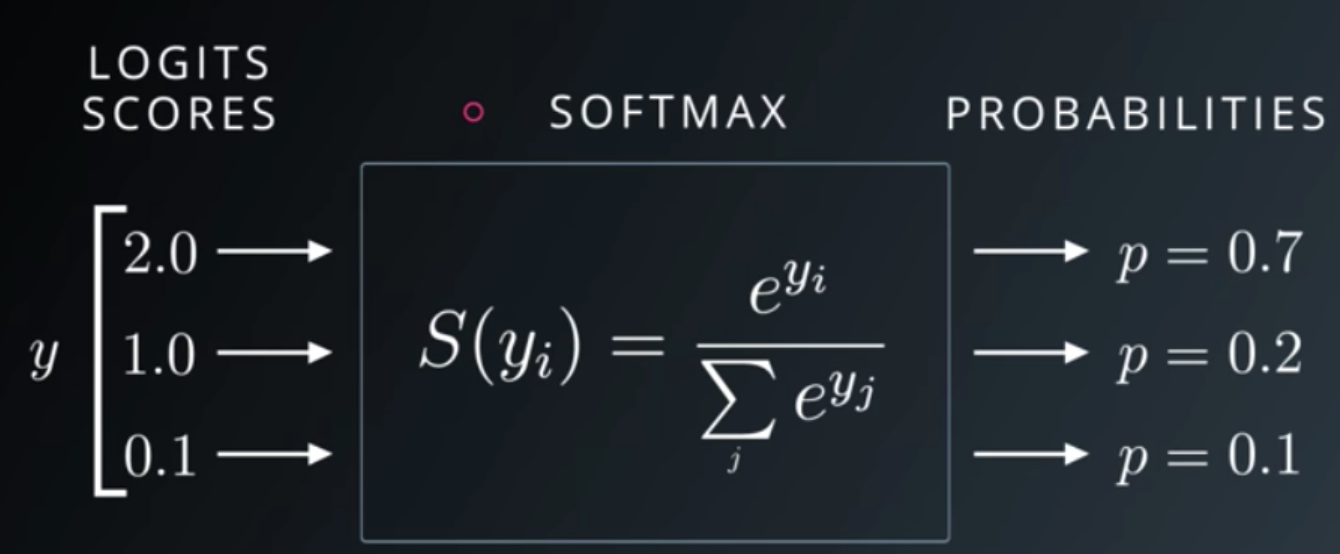
\includegraphics[width=8cm]{./figures/softmax function}
\caption{Softmax function pushing high scores close to 1 and low scores close to 0}
\end{figure}

The final layer in our model is also a fully-connected layer but it is 
special. The number of units is the number of classes, in our case, 26. The 
activation function used is softmax activation, it gives a probability 
distribution wherein a value is pushed close to 1 if it is large or close to 0 
if it is small.

\subsection{Train Phase}

The training phase consists of four steps:
\begin{enumerate}
	\item Input: get \gls{roi} of shape \texttt{[250×250×3]} from image
	\item Transfer learning: get the model activations from last layer
	\item Train model: recognize \gls{asl} alphabet using previous activations
	\item Repeat: process batches by resuming the training in each iteration
\end{enumerate}

\begin{figure}[h]
\centering
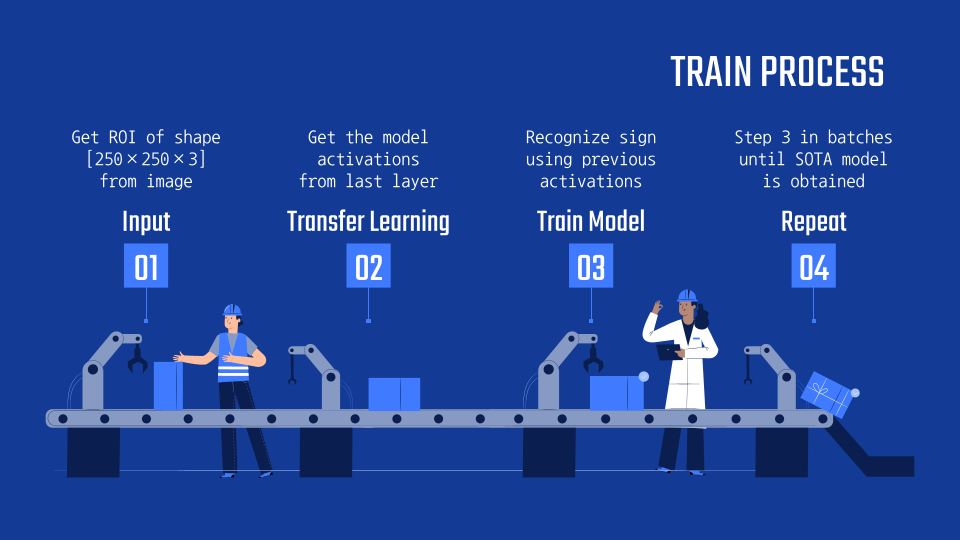
\includegraphics[width=8cm]{./figures/train process}
\caption{Process of training the model}
\end{figure}


\section{Experimental Results}

\subsection{Predict Phase}

The predict phase is exactly the same as the train phase except for the last 
step:
\begin{itemize}
	\item Predict: display the alphabet with the highest score
\end{itemize}

\begin{figure}[h]
\centering
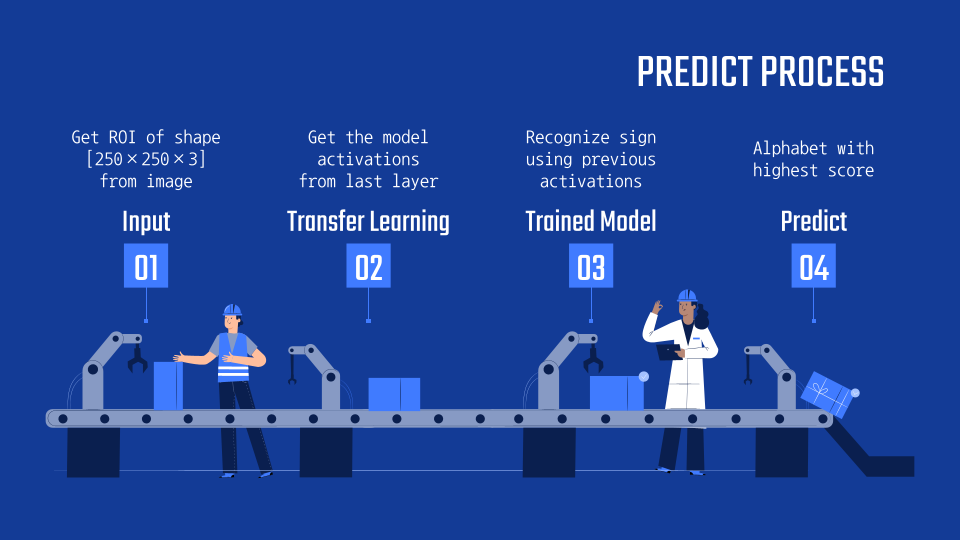
\includegraphics[width=8cm]{./figures/predict process}
\caption{Process of testing the model}
\end{figure}

\subsection{Model Statistics}

When we see the performance for the trained model, we see \inception 
outperforms them all. This again can be explained by its very efficient 
architecture which is unlike its predecessors. Peculiarly, \resnet which had 
the best overall performance on the ImageNet dataset, has the worst 
performance on our dataset. The reason for this is unclear, perhaps an 
in-depth analysis of the weights can give a valid explanation. Due to the 
small range of labels to classify, i.e., 24, \mobilenet performs very well as 
its light-weight architecture can easily handle the small corpus of signs. 
\xception also works well but its better to use \mobilenet due to its 
computational advantage.

\begin{table}[h]
\begin{tabular}{ |l|c|c|c| }
	\hline
	\textbf{Model} & \textbf{Size} & \textbf{Accuracy} & \textbf{Parameters} \\ \hline
	\mobilenet & 91 MB & 0.918 & 7,934,872 \\ \hline
	\inception & 99 MB & 0.924 & 8,598,424 \\ \hline
	\xception & 100 MB & 0.908 & 8,721,304 \\ \hline
	\resnet & 93 MB & 0.848 & 8,074,136 \\
	\hline
\end{tabular}
\caption{Trained model statistics using varying transfer learning models}
\end{table}

The overall performance of the model on the test dataset is \textbf{92.36\%} 
which works well. The performance can further be improved by using the idea of 
model ensembling which uses the results of the multiple models together to get 
a combined prediction. This often works better than using an individual model 
since each model has its own best-side or data that it can recognize well 
leading to good performance.

\subsection{Model Performance}

The model was evaluated and tested on all 24 alphabets of \gls{asl}. From the 
results shown in \autoref{asl abcdef} it is clear that the model performs 
well. On further testing, it was found that specific signs such as the letter 
\textit{F} are easily recognizable on the \inception or the letter \textit{U} 
on the \xception model. This could just be due to the difference in the 
architecture. \mobilenet works well overall and is fast when compared to the 
other models. All the models work in real-time and work even better with good 
lighting and clear backgrounds.

\begin{figure}[h]
\centering
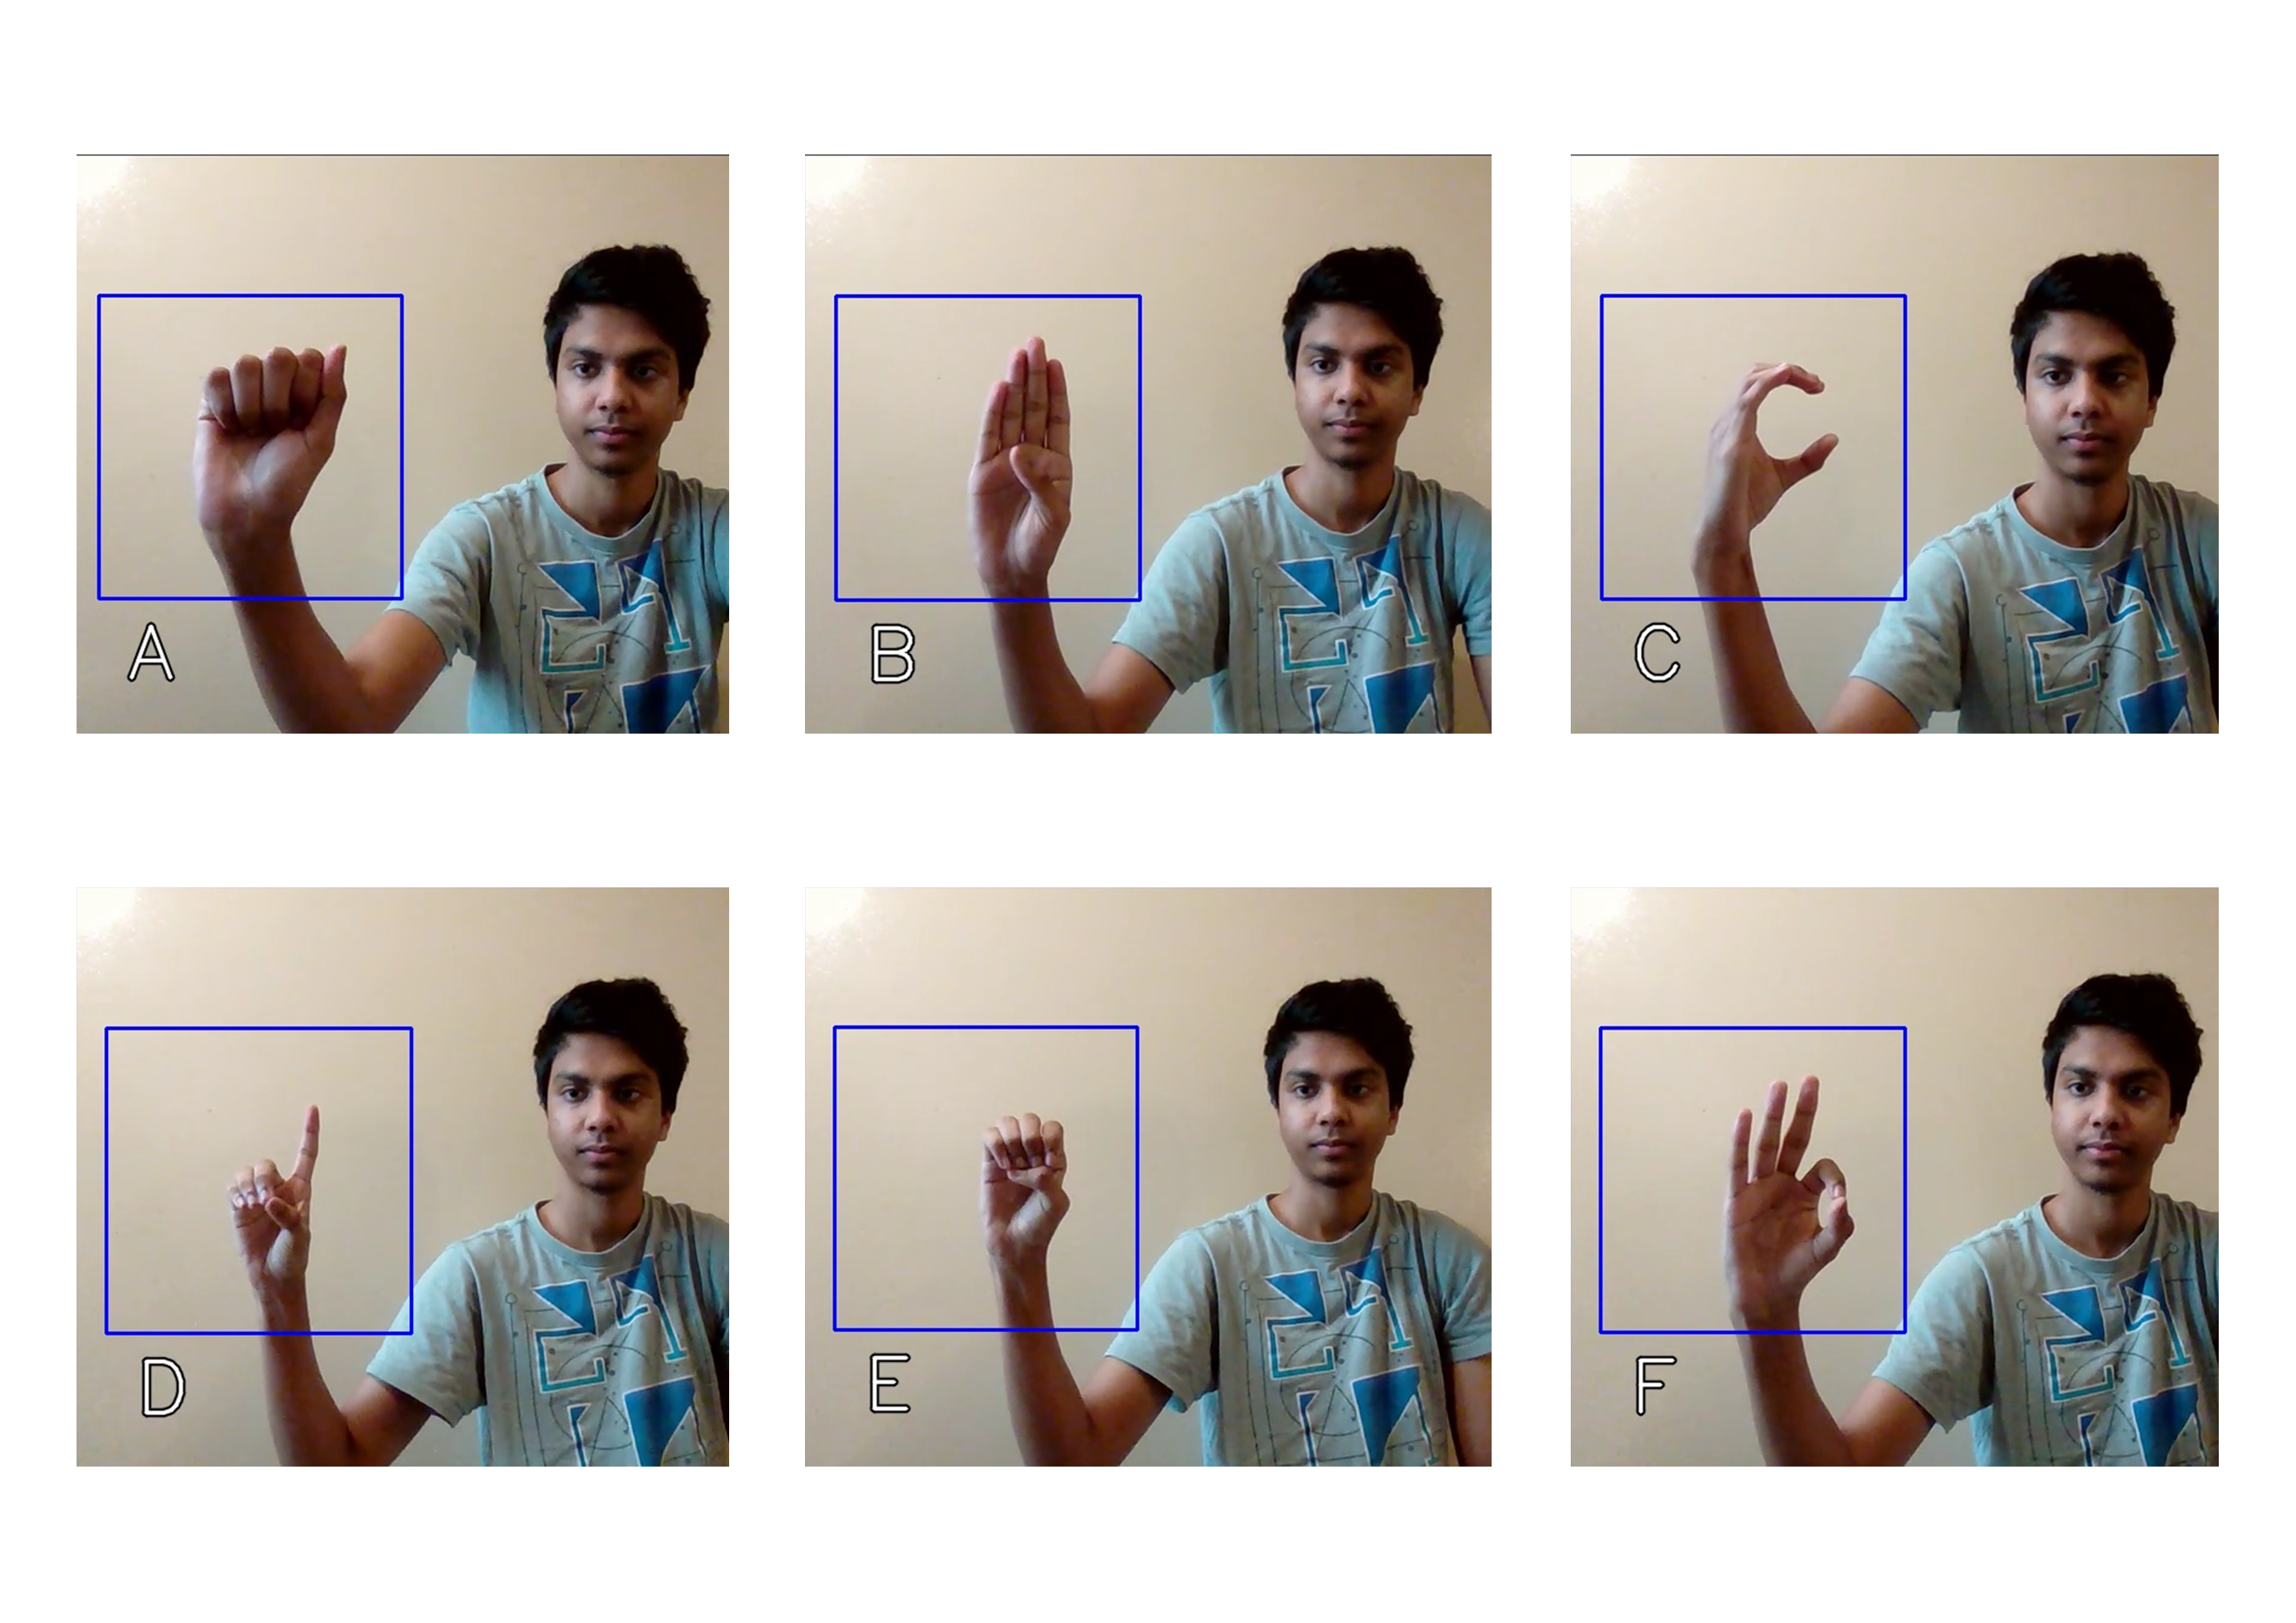
\includegraphics[width=8cm]{./figures/asl abcdef}
\caption{Prediction of the alphabets A, B, C, D, E, and F}
\label{asl abcdef}
\end{figure}

But things are not always perfect as shown in \autoref{asl ddc}, some of the 
letters in \gls{asl} are similar causing discrepancies and confusion when 
given as input to the model. The distribution is shown below:
\begin{itemize}
	\item M, N, T
	\item D, R, U
	\item G, H
	\item A, E, S
	\item C, O, X
\end{itemize}

\begin{figure}[h]
\centering
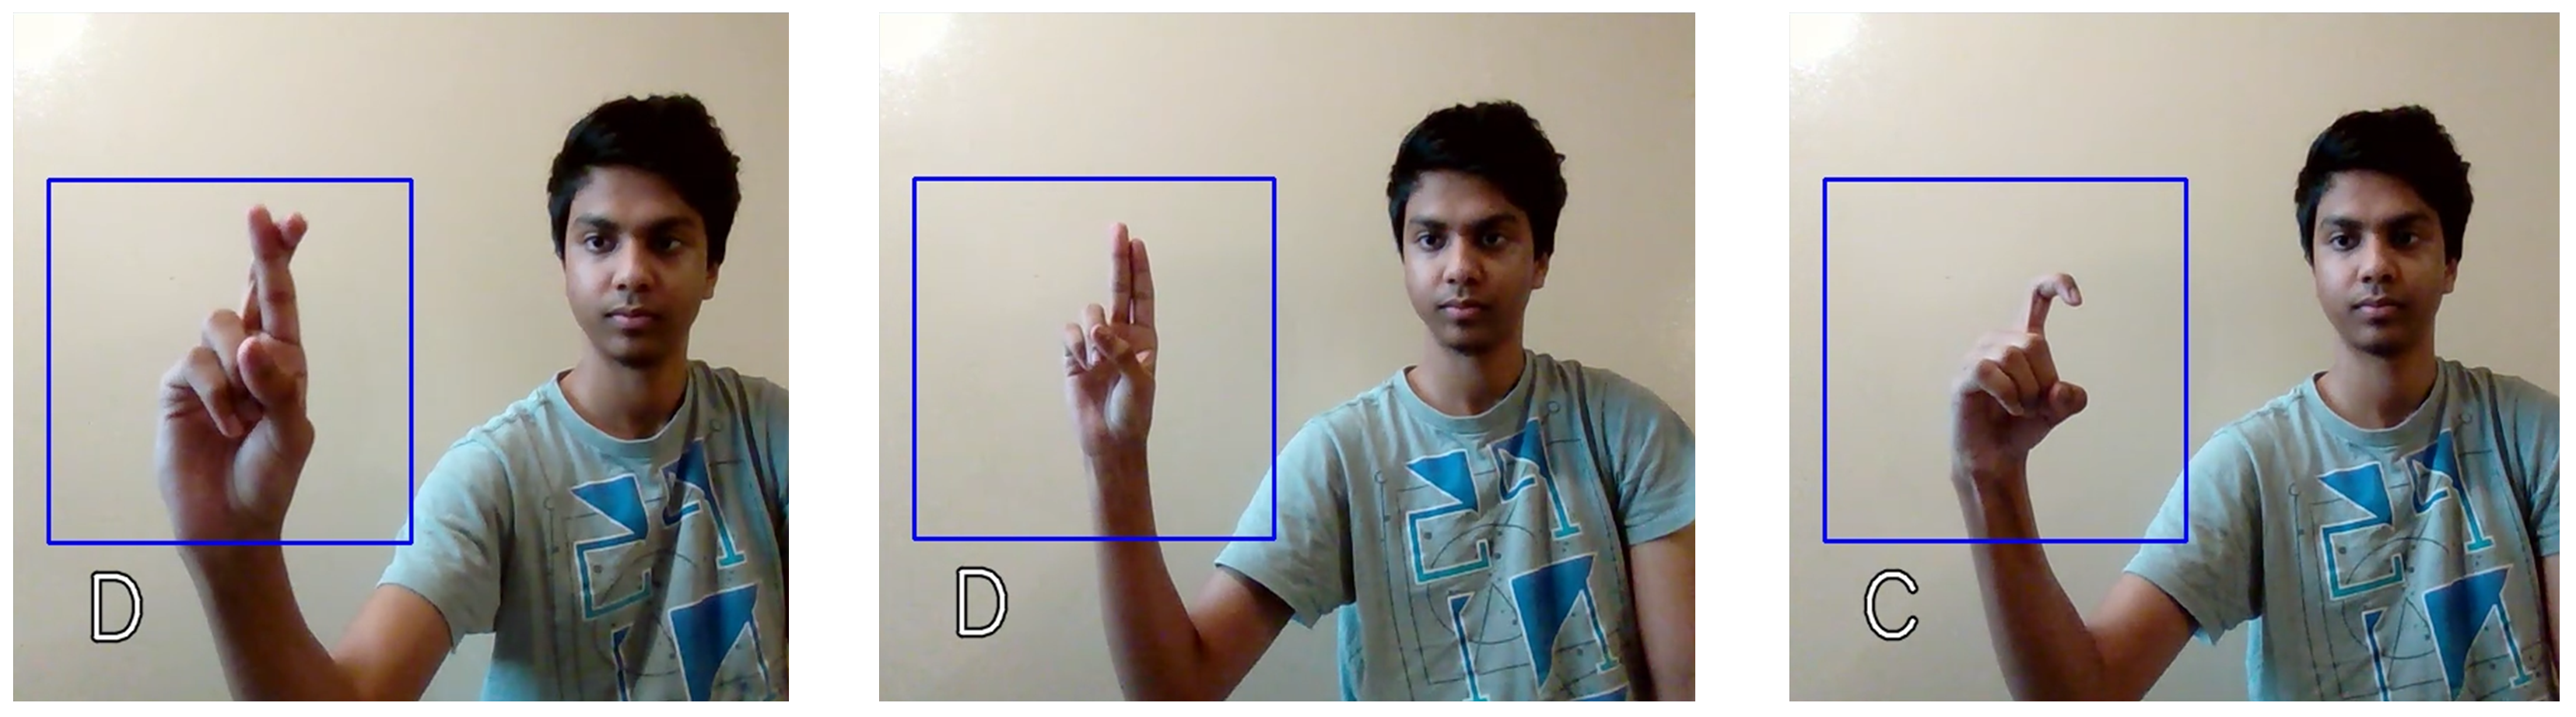
\includegraphics[width=8cm]{./figures/asl ddc}
\caption{Incorrect prediction of R as D, U as D, and X as C}
\label{asl ddc}
\end{figure}

Most of the time, the incorrect results fall in the similar categories due to the confusion caused by high similarities. Looking closely at the distribution of \texttt{{M, N, T}}, we see all of them just differ in the position of the thumb in between the other fingers. Again, the performance can be improved by adding more variability into the dataset and improving the training model architecture.


\section{Conclusion}

\subsection{Results}

We successfully created a model to make fingerspelling in \gls{asl} possible 
without the need of sophisticated components or expensive hardware. In 
conclusion:

\begin{itemize}
	\item 466,000 people have disabling hearing loss.
	\item Achieved a high accuracy of \textbf{92.36\%} on the test dataset.
	\item Successfully fingerspell the 24 static alphabets of \gls{asl}.
	\item Provide four transfer learning models for user flexibility.
\end{itemize}

Most importantly, the model is fast, and it runs on your smartphone in 
real-time. I hope this project helps us bridge the gap and get us closer to 
breaking the communication barrier.

\subsection{Future Work}

A couple of approaches could be used to increase the performance of the model:

\begin{itemize}
	\item Model Ensembling: use results of multiple models to output the 
	predicted letter.
	\item Tree Algorithms: random forest works well for classification tasks.
	\item Hidden Markov: a statistical model which learns by observing.
\end{itemize}

Our recommendations:

\begin{itemize}
	\item Number of categories: increase the corpus of signs being classified 
	from 24 alphabets to words and gestures.
	\item Software: integrate model into mobile, web, and desktop app allowing 
	it to be more wide-spread and distributed.
	\item Motion: classify more than just static signs and build over to dynamic 
	signs requiring motion.
\end{itemize}


\bibliographystyle{ieeetr}
\bibliography{biblio}

\listoffigures
\listoftables

\glsaddall
\setlength{\glsdescwidth}{0.8\textwidth}
\printglossary[type=\acronymtype,title=List Of Abbreviations]

% (TODO: use a clearer way to separate)
\clearpage
\LARGE{\textbf{Additional Resources}}

\begin{figure}[h]
\centering
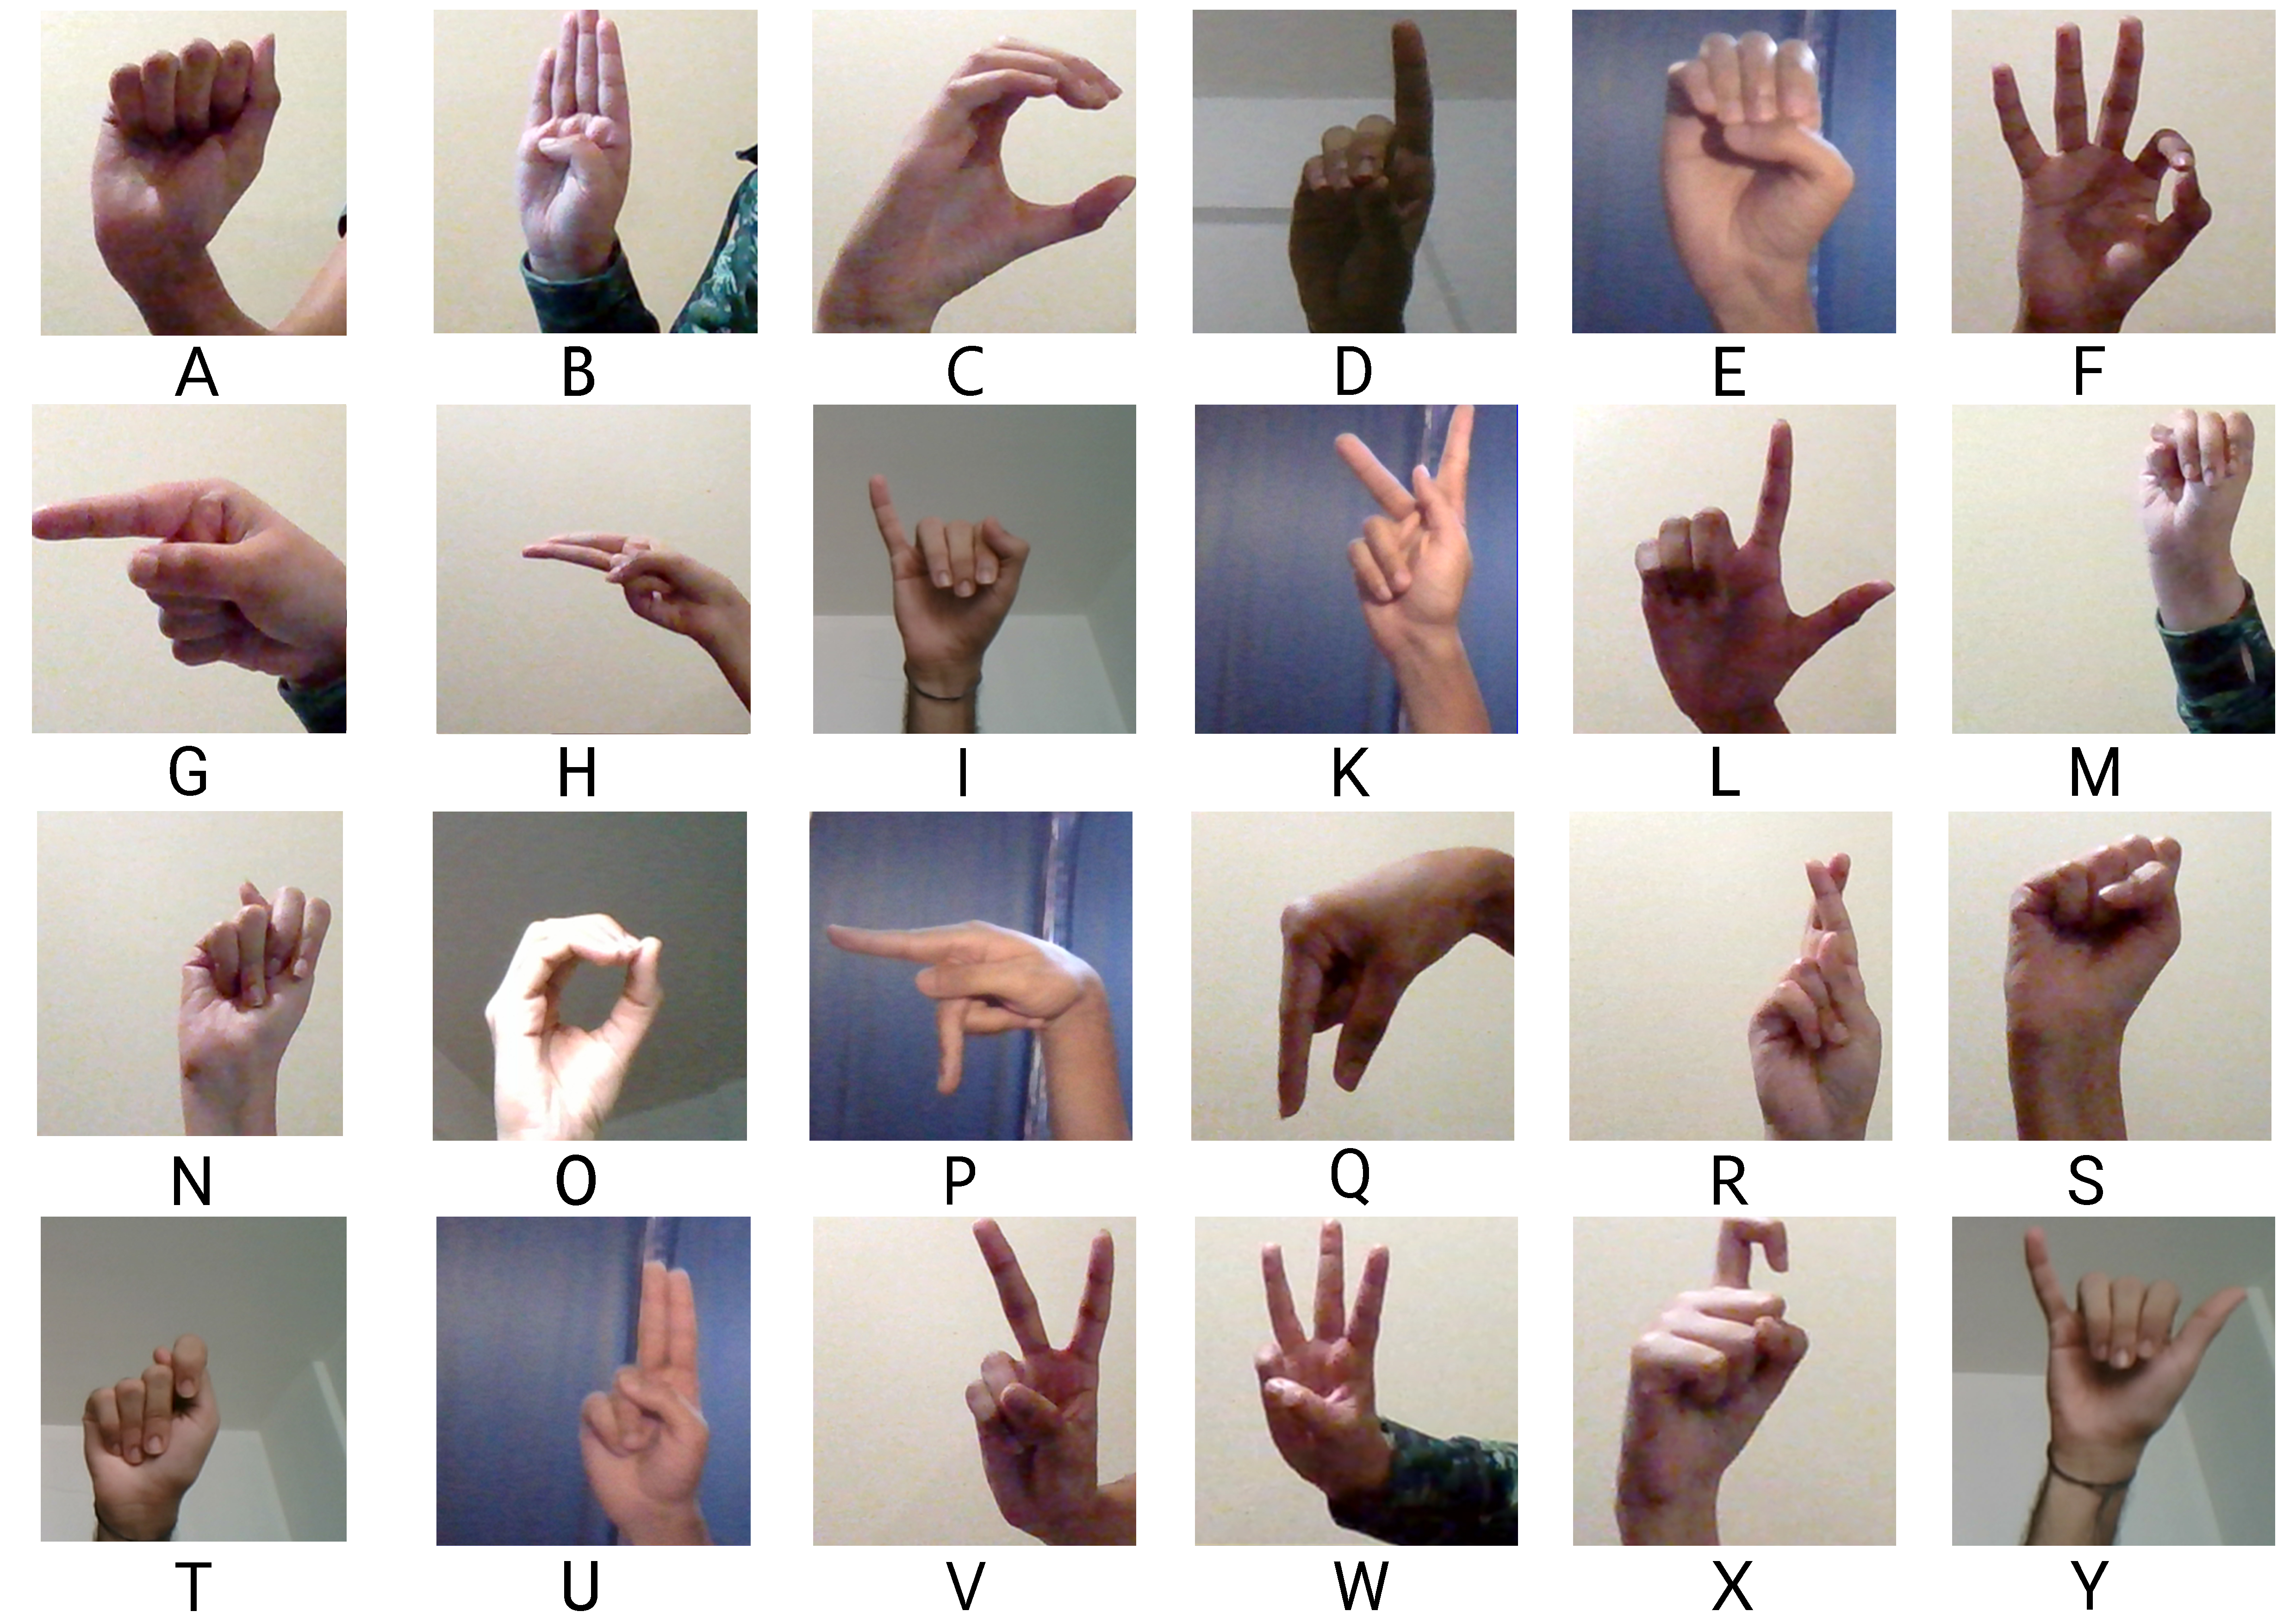
\includegraphics[width=8cm]{./figures/alphabets}
\caption{ASL alphabets from our dataset}
\end{figure}

\begin{figure}[h]
\centering
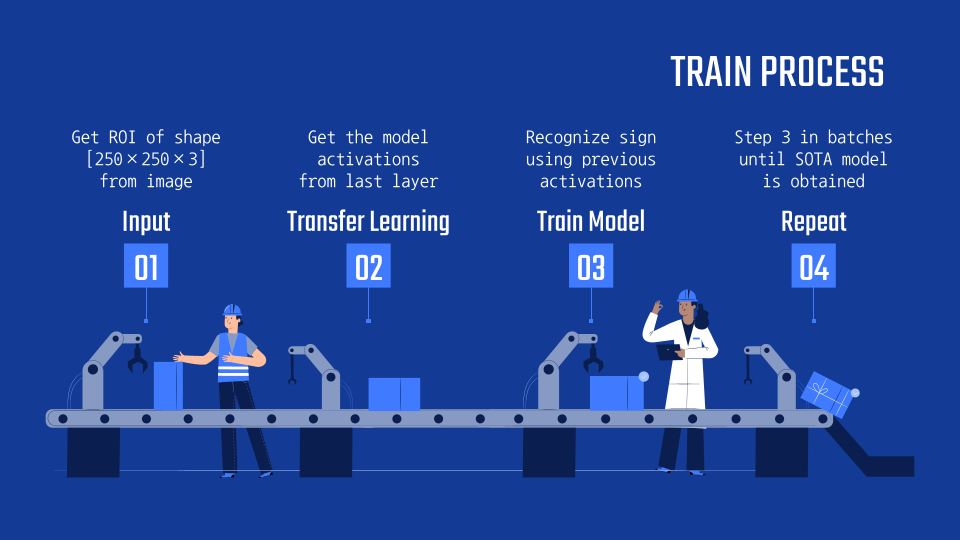
\includegraphics[width=8cm]{./figures/train process}
\caption{Process of training the model}
\end{figure}

\begin{figure}[h]
\centering
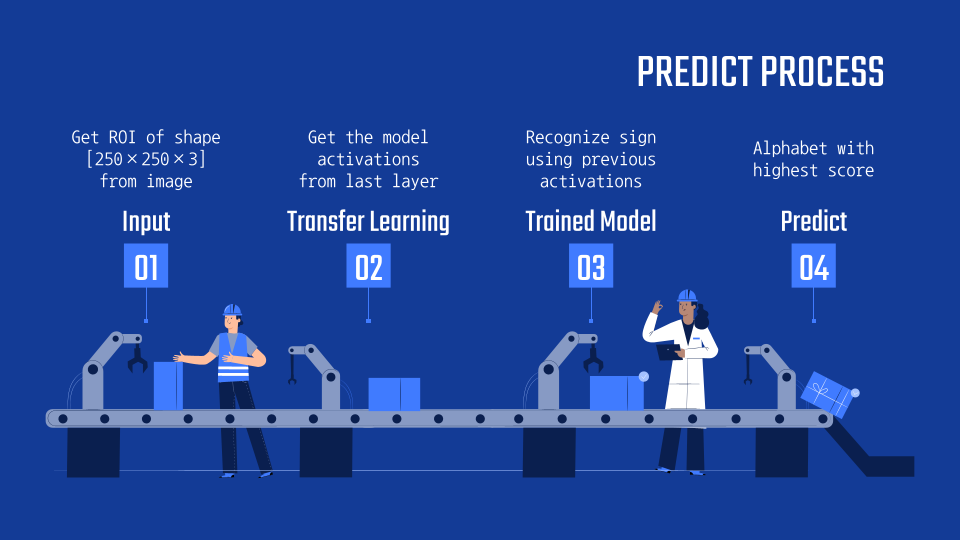
\includegraphics[width=8cm]{./figures/predict process}
\caption{Process of testing the model}
\end{figure}

% (TODO: use a clearer way to separate)
\clearpage

% (TODO: use a clearer way to separate)
\clearpage

\begin{table}[h]
\begin{tabular}{ | @{\makebox[2em][r]{\rownumber\space}} |l|c| }
	\hline
	\multicolumn{1}{ | @{\makebox[2em][r]{\textbf{ ID }}} |l| }{\textbf{Layer (Type)}} 
	& \multicolumn{1}{ |c| }{\textbf{Number of Parameters}} \\ \hline
	\texttt{dense\_1 (Dense)} & \emph{dependent} \\ \hline
	\texttt{dense\_2 (Dense)} & 524,800 \\ \hline
	\texttt{dense\_3 (Dense)} & 131,328 \\ \hline
	\texttt{dense\_4 (Dense)} & 32,896 \\ \hline
	\texttt{up\_sampling2d\_1 (UpSampling2D)} & 0 \\ \hline
	\texttt{conv2d\_5 (Conv2D)} & 131,136 \\ \hline
	\texttt{depthwise\_conv2d\_1 (DepthwiseConv2D)} & 1,088 \\ \hline
	\texttt{up\_sampling2d\_2 (UpSampling2D)} & 0 \\ \hline
	\texttt{depthwise\_conv2d\_2 (DepthwiseConv2D)} & 1,088 \\ \hline
	\texttt{conv2d\_6 (Conv2D)} & 65,600 \\ \hline
	\texttt{dense\_5 (Dense)} & 8,320 \\ \hline
	\texttt{dense\_6 (Dense)} & 33,024 \\ \hline
	\texttt{dense\_7 (Dense)} & 131,584 \\ \hline
	\texttt{dense\_8 (Dense)} & 525,312 \\ \hline
	\texttt{dense\_9 (Dense)} & 2,099,200 \\ \hline
	\texttt{dense\_10 (Dense)} & 2,098,176 \\ \hline
	\texttt{dense\_11 (Dense)} & 524,800 \\ \hline
	\texttt{dense\_12 (Dense)} & 131,328 \\ \hline
	\texttt{dense\_13 (Dense)} & 32,896 \\ \hline
	\texttt{max\_pooling2d\_1 (MaxPooling2D)} & 0 \\ \hline
	\texttt{flatten\_1 (Flatten)} & 0 \\ \hline
	\texttt{dense\_14 (Dense)} & \emph{dependent} \\
	\hline
\end{tabular}
\caption{Model architecture and number of parameters in each layer}
\end{table}

% (TODO: use a clearer way to separate)
\clearpage

\begin{table}[h]
\begin{tabular}{ | @{\makebox[2em][r]{\rownumber\space}} |l|l| }
	\hline
	\multicolumn{1}{ | @{\makebox[2em][r]{\textbf{ ID }}} |l| }{\textbf{Layer (Type)}}
	& \multicolumn{1}{ |c| }{\textbf{Number of Parameters}} \\ \hline
	\texttt{(None, 8, 8, 1024)} & \texttt{(None, 6, 6, 1024)} \\ \hline
	\texttt{(None, 8, 8, 512)} & \texttt{(None, 6, 6, 512)} \\ \hline
	\texttt{(None, 8, 8, 256)} & \texttt{(None, 6, 6, 256)} \\ \hline
	\texttt{(None, 8, 8, 128)} & \texttt{(None, 6, 6, 128)} \\ \hline
	\texttt{(None, 16, 16, 128)} & \texttt{(None, 12, 12, 128)} \\ \hline
	\texttt{(None, 13, 13, 64)} & \texttt{(None, 9, 9, 64)} \\ \hline
	\texttt{(None, 10, 10, 64)} & \texttt{(None, 6, 6, 64)} \\ \hline
	\texttt{(None, 20, 20, 64)} & \texttt{(None, 12, 12, 64)} \\ \hline
	\texttt{(None, 17, 17, 64)} & \texttt{(None, 9, 9, 64)} \\ \hline
	\texttt{(None, 14, 14, 64)} & \texttt{(None, 6, 6, 64)} \\ \hline
	\texttt{(None, 14, 14, 128)} & \texttt{(None, 6, 6, 128)} \\ \hline
	\texttt{(None, 14, 14, 256)} & \texttt{(None, 6, 6, 256)} \\ \hline
	\texttt{(None, 14, 14, 512)} & \texttt{(None, 6, 6, 512)} \\ \hline
	\texttt{(None, 14, 14, 1024)} & \texttt{(None, 6, 6, 1024)} \\ \hline
	\texttt{(None, 14, 14, 2048)} & \texttt{(None, 6, 6, 2048)} \\ \hline
	\texttt{(None, 14, 14, 1024)} & \texttt{(None, 6, 6, 1024)} \\ \hline
	\texttt{(None, 14, 14, 512)} & \texttt{(None, 6, 6, 512)} \\ \hline
	\texttt{(None, 14, 14, 256)} & \texttt{(None, 6, 6, 256)} \\ \hline
	\texttt{(None, 14, 14, 128)} & \texttt{(None, 6, 6, 128)} \\ \hline
	\texttt{(None, 7, 7, 128)} & \texttt{(None, 3, 3, 128)} \\ \hline
	\texttt{(None, 6272)} & \texttt{(None, 1152)} \\ \hline
	\texttt{(None, 24)} & \\
	\hline
\end{tabular}
\caption{Shape of each layer in trained model for different transfer learning models}
\end{table}

\end{document}
